\chapter{Platforma Zynq-7000}
\label{cha:platform}

Karta uruchomieniowa ZYBO jest przedstawicielem rodziny układów SoC (\emph{ang}. System-on-a-chip) Zynq-7000. %TODO ZYBO to jest karta uruchomieniowa/ewaluacyjna, układ Zynq. Trzeba to rozróżnić.
% OK
SoC to układy scalone integrujące zbiór układów elektronicznych, takich jak mikroprocesor, układy koprocesujące, interfejsy wejścia i wyjścia, czy pamięci. Są one powszechnie wykorzystywane do projektowania systemów wbudowanych. %TODO wszystkie elementy budowy ??? inaczej to trzeba napisać...
% OK?
Centralną część układu rodziny Zynq-7000 stanowi dwurdzeniowy procesor o architekturze ARM w wersji Cortex-A9, współpracujący z działającym równolegle układem FPGA, opartym na architekturze Artix-7 lub Kintex-7. \cite{zynq-homepage} %TODO proszę zwrócić uwagę, że \cite powinno być przed kropką. Nie wspomniał Pan o logice programowalnej. 
% OK, poprawię masowo po 1. korekcie
Są to układy heterogeniczne, łączące w sobie elementy klasycznego układu FPGA (\emph{PL}, \emph{ang.} Programmable Logic) oraz procesora ARM (\emph{PS}, \emph{ang.} Processing System). %TODO to zdanie jest powt. wcześniejszego - jakoś trzeba to zintegrować.
% OK

Karta ZYBO wyposażona jest ponadto w 512 MB pamięci RAM, złącza HDMI i VGA do transmisji obrazu, gniazda Jack do przesyłu sygnału dźwiękowego, gniazdo USB oraz slot pamięci MicroSD. %TODO Karta ZYBO, dzwięku -> sygnału dźwiękowego
% OK
Komunikacja sieciowa jest możliwa dzięki implementacji stosu TCP/IP i obecności gniazda RJ-45. \cite{zynq-datasheet}

Układy rodziny Zynq-7000 są stosowane w aplikacjach systemów wsparcia kierowców, systemach wizyjnych wysokich rozdzielczości, cyfrowego przetwarzania sygnałów czy kryptograficznych. Zaproponowano wykorzystanie zalet elementów FPGA i CPU do projektowania systemów wsparcia kierowców ADAS, co pozwoliło na redukcję czasu odpowiedzi systemu i zapotrzebowania na energię. \cite{GuanwenZhong}
W innej pracy zbadano możliwość wykorzystania układu do transmisji sygnału o rozdzielczości 4K ($3840 \times 2160$ pikseli) przy możliwie niewielkim zużyciu zasobów i energii. \cite{MaleenAbeydeera}
Wśród zagadnień kryptograficznych, realizowanych przy użyciu omawianej rodziny układu wymienić można algorytmy generowania liczb pseudolosowych o wysokiej rozdzielczości.	\cite{PawelDabal2014} %TODO (po kropce) poza tym moze o jedno zdadnie wiecej na temat kazdego artykuły i inny układ (nie na końcu, a po zdaniu cite)
% OK

Na rysunku \ref{fig:zynq-overview} przedstawiono schemat omawianej architektury.

\begin{figure}[h]
	\centering
	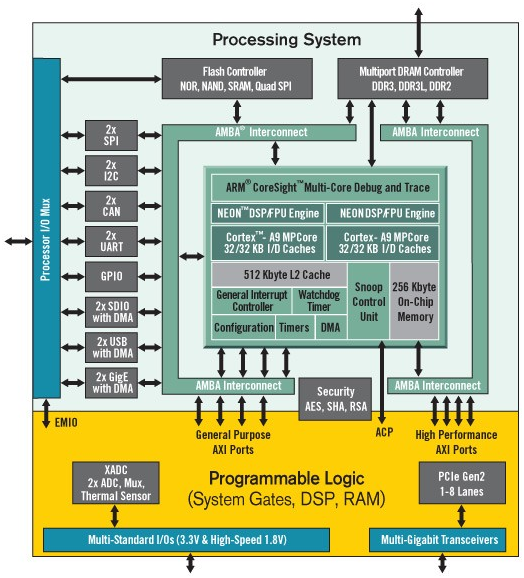
\includegraphics[width=12cm]{img/zyng-platform.png}
	\caption{Schemat architektury Zynq-7000. (Źródło: \cite{zybo-reference-manual})}
	\label{fig:zynq-overview}
\end{figure}
%TODO może nieco większy
% OK

Schemat przedstawia podział układu na części \emph{PL} -- oznaczonej kolorem żółtym, oraz \emph{PS} -- na zielono.
Architektura części programowalnej zbliżona jest do powszechnie stosowanych układów FPGA. %TODO konkretnie jaka seria Xilinx
% dodałem tę informację nieco wyżej
Wyposażono ją jednak w zbiór portów umożliwiających wydajną komunikację z procesorem. 
Ponadto, konfiguracja tej części wykonywana jest na starcie przez procesor lub przy użyciu interfejsu JTAG i układ nie zawiera elementów pozwalających na wykorzystanie logiki programowalnej niezależnie.
Część procesorowa wyposażona jest w szereg interfejsów, w tym kontroler pamięci DDR3, interfejs komunikacji AMBA oraz zbiór interfejsów peryferyjnych.

Procesor wyposażony jest w koprocesor arytmetyczny (\emph{FPU}), wspierający w obliczeniach na liczbach zmiennoprzecinkowych oraz wspiera obsługę architektury SIMD (\emph{ang.} Single Instruction, Multiple Data) -- pozwalającej na przetwarzanie wielu strumieni danych przy użyciu jednego strumienia instrukcji. 
Zagadnienia te szerzej opisane zostały w sekcji \ref{sec:arm-neon}.
%TODO Tu dobrze by było się odwoływać do nazw bloków z rysunku (np. FPU).
% OK

Układ wyposażony jest w kontroler pamięci DDR, obsługujący żądania dostępu ze strony zarówno procesora, jak i logiki programowalnej. %TODO logiki programowalnej (bez powt. układ)
% OK
Pamięć jest współdzielona między obiema częściami. %TODO obiema częściami
% OK
Pozwala to na wymianę danych, do czego wykorzystywany jest standard AXI. Zastosowanie znajduje również mechanizm DMA, pozwalający na przeprowadzanie operacji z użyciem pamięci bez udziału procesora. 
Interfejs pozwala na transmisję pojedynczych słów danych, umożliwiając konfigurację parametrów pracy modułów algorytmicznych, jak i na transmisję o wysokiej przepustowości. 
Pozwala to, dzięki zastosowaniu modułu VDMA, na przesyłanie obrazu o rozdzielczości HD z częstotliwością osiągającą wartości 680 klatek na sekundę  \cite{axi-vdma-guide}. 
Interfejs AXI opisano szerzej w sekcji \ref{sec:axi-std}.

Dzięki zastosowaniu kontrolera przerwań (\emph{General Interrupt Controller}) możliwe jest wykorzystanie modułów logiki programowalnej komunikujących się z procesorem z wykorzystaniem techniki zgłaszania żądań. Zagadnienie to opisano w sekcji \ref{sec:axi-interrupts}.

Ponadto, dostępne są powszechnie spotykane układy zegarowe (\emph{Timers}) i \emph{Watchdog}, odpowiedzialny za przerwanie pracy procesora w przypadku wykrycia błędnego wykonania programu.

Kontekst pamięciowy synchronizowany jest pomiędzy oboma rdzeniami procesora dzięki modułowi \emph{Snoop Control Unit}.

Układ logiki programowalnej należeć może do rodzin Artix-7 lub Kintex-7 i zbudowany jest z typowych elementów wykorzystywanych w FPGA o różnej liczebności, związanej z klasą układu:
\begin{itemize}
	\item CLB (\emph{ang.} Configurable Logic Blocks) -- w tym tablice Look-up (\emph{LUT}) -- $14400 - 277400$ elementów, przerzutniki (\emph{FF}) -- $28800 - 554800$ elementów.
	
	\item Pamięci \emph{Block RAM} -- od $1,8Mb$ do $26,5Mb$ ($50 - 755$ elementów).
	
	\item Elementy \emph{DSP} -- wykorzystywane zwykle do implementacji operacji dodawania i mnożenia -- $66 - 2020$ elementów.
	
	\item Bloki \emph{IOB} -- umożliwiające budowę interfejsów wejściowych i wyjściowych.
	
	\item Inne -- w tym interfejs JTAG, PCI Express czy konwertery analogowo-cyfrowe.
\end{itemize}
%TODO Brakuje choćby podstawowego opisu zasobów PL - dodać.
% OK dodałem opis
%TODO Proszę dodać opisy pozostałych elementów PS (choć 1-2 zdania na każdy bloczek)
% OK, dodałem te, które mogą być jakkolwiek istotne z mojej perspektywy.
%TODO Proszę napisać, dlaczego AXI i FPU opisane są później... 
% nie chciałem rozdzielać tych zagadnień na część teoretyczną i praktyczną. Wg mnie nie miałoby to sensu zwłaszcza dla FPU.

%TODO TO bym jakoś bardziej w kierunku rozdziału o systemach operacyjnych przekształcił (bo de facto o tym jest). Tylko wtedy Peta i inne to subsection (przeorganizować hierarchię)
% OK, poprawiłem
\section{Zastosowanie systemu operacyjnego}
\label{sec:arm-programming}

Centralny element architektury stanowi dwurdzeniowy procesor ARM. 
Jest on odpowiedzialny za przeprowadzenie konfiguracji logiki reprogramowalnej. 
Ponadto pozwala na wykonanie dowolnego programu użytkownika. 
Powszechnie stosowana jest konfiguracja \textit{bare-metal}, w której procesor wykonuje program zaprojektowany w pełni przez użytkownika. 
Pozwala to na uzyskanie możliwie największej kontroli nad pracą układu, ogranicza jednak możliwości wykorzystania pełni zasobów procesora oraz utrudnia projektowanie rozbudowanych aplikacji. Brak systemu operacyjnego ogranicza możliwość wykorzystania komunikacji sieciowej na etapie wykonania programu. Możliwości przechowywania wyników i logów aplikacji są niewielkie. Ponadto, użycie zewnętrznych bibliotek, w tym związanych z przetwarzaniem obrazów, takich jak OpenCV, jest niemożliwa. W efekcie, wykorzystanie konfiguracji pozbawionej systemu operacyjnego nie jest możliwe w przypadku aplikacji wymagających nadzoru bez fizycznego dostępu do układu czy przechowywania wyników.
%TODO może nieco więcej szczegółów i przede wszstykim, że brak OS.
% OK

W niniejszej pracy badano możliwość wykorzystania systemu operacyjnego Linux na przykładzie aplikacji systemów wizyjnych. 
Dzięki zastosowaniu Linuxa, możliwe staje się budowanie programów składających się z wielu modułów działających niezależnie. 
System ten wspiera obsługę sieci, co pozwala na wykorzystanie narzędzi komunikacji sieciowej, jak SSH \cite{ssh-protocol}, do konfiguracji i nadzorowania działania aplikacji, co opisano w rozdziale \ref{sec:ssh}. 
Ponadto, możliwe jest wykorzystanie powszechnie dostępnych bibliotek, ułatwiających rozwój aplikacji w krótkim czasie. 
Zagadnienie to badano na przykładzie biblioteki OpenCV \cite{opencv-library}, udostępniającej narzędzia przetwarzania obrazów, co opisano w rozdziale \ref{sec:opencv-lib}.

Zbadano możliwość wykorzystania systemu PetaLinux, rozwijanego przez organizację Xilinx, jak i podstawowej wersji systemu, opartej wyłącznie na źródle jądra, oraz dystrybucji bazującej na Ubuntu Core. %TODO co jest rozumiane przed podstawową wersję systemu ?
% OK?
Ponadto, rozpatrzono możliwość użycia systemu czasu rzeczywistego do wykonania zadań obliczeniowych z zachowaniem reżimu czasowego.
%TODO Wspomnieć o RTOS
% OK

\subsection{PetaLinux} %TODO Sub
% OK

Firma Xilinx zapewnia dostęp do zbioru narzędzi \emph{PetaLinux Tools} \cite{petalinux-tools} umożliwiających przeprowadzenie procesu konfiguracji, budowania i uruchamiania systemu Linux na platformie Zynq. 
Dzięki zintegrowaniu koniecznych narzędzi w jednym pakiecie, proces ten jest w dużej części zautomatyzowany i ogranicza interakcję z programistą, zapewniając przy tym możliwość dowolnej konfiguracji systemu.

Celem wykorzystania omawianego pakietu narzędzi jest zbudowanie systemu operacyjnego gotowego do uruchomienia i umożliwiającego szybką rekonfirugację zarówno elementów logiki reprogramowalnej jak i samego systemu operacyjnego.

Pakiet wymaga dostarczenia zewnętrznych zależności, w tym narzędzi umożliwiających budowanie systemu -- kompilatora, generatora parserów, systemu budowania -- oraz zbioru narzędzi programistycznych i konfiguracyjnych.
W przypadku dystrybucji Debian, zależności mogą być zainstalowane poleceniem:

\begin{lstlisting}[breaklines=true]
apt-get install tofrodos iproute2 gawk gcc git make net-tools libncurses5-dev tftpd zlib1g-dev libssl-dev flex bison libselinux1
\end{lstlisting}

W przypadku pracy na systemie wspierającym architekturę 64-bitową, konieczne jest również zainstalowanie bibliotek programistycznych dla architektury 32-bitowej.

\begin{lstlisting}[breaklines=true]
dpkg --add-architecture i386
apt-get update
apt-get install libc6:i386 libncurses5:i386 libstdc++6:i386
apt-get install libgtk2.0-0:i386 libxtst6:i386 gtk2-engines-murrine:i386 lib32stdc++6 libxt6:i386 libdbus-glib-1-2:i386 libasound2:i386
\end{lstlisting}

Praca z pakietem wymaga ponadto wykorzystania oprogramowania \emph{Vivado Design Suite} \cite{vivado-home} do zaprojektowania układu połączeń logiki reprogramowalnej oraz \emph{Xilinx SDK} \cite{xsdk-home} do kompilacji programów uruchamianych w środowisku systemu operacyjnego układu.

Pierwszym krokiem jest wykonanie projektu w pakiecie \emph{Vivado}. 
Szczegóły procesu opisano w sekcji \ref{sec:vivado-conf}. %TODO sekcji -> rozdziale (wydaje mi się, ze w PL słowo sekcja nie powinno być uzywane w tym kontekście - kalka z ENG)
% OK, poprawię masowo w całej pracy na końcu 1. korekty
Wyeksportowany projekt Vivado jest konieczny do przeprowadzenia procesu budowania systemu, proces konfiguracji projektu PetaLinux opisano w sekcji \ref{sec:petalinux-config}. %TODO akapity jednozdaniowe są zakazane...
% OK, spróbuję je wyłapać

Pakiet udostępnia możliwość dodania do budowanego systemu zbioru programów i bibliotek. 
Dostępne jest kilkaset pakietów oprogramowania oferowanych na zasadach wolnych licencji, w tym biblioteki do przetwarzania obrazów. %TODO Dostępne, dostępnego
% OK
Ponadto, pakiet umożliwia dodanie własnoręcznie zbudowanych aplikacji. 
Pozwala to na integrację etapu projektowania aplikacji oraz budowy i uruchamiania systemu operacyjnego w jednym procesie.

Projekt PetaLinux jest niezależny od projektu Vivado i może powstawać równolegle. 
Zmiany w strukturze modułów logiki reprogramowalnej wymagają ponownego zbudowania plików wynikowych systemu operacyjnego PetaLinux, jednak proces ten został wydzielony z oprogramowania Vivado. %TODO co tu jest rozumiane przez system
% OK
Pozwala to na wykorzystanie jednego projektu opisującego logikę współpracującego z aplikacjami bare metal i systemowymi. 

Proces budowania systemu jest czasochłonny, na etapie prototypowania aplikacji praktyczne jest zastosowanie oprogramowania pracującego w trybie bare-metal. %TODO bare-metal - pisałbym w \textit{} 
% OK, poprawię masowo na koniec
Pozwala to na przeprowadzanie procesu debugowania aplikacji bezpośrednio z poziomu oprogramowania Vivado/SDK. 
Po upewnieniu się, że sprzętowa część algorytmu działa poprawnie, zaprojektować można aplikację systemową, odpowiedzialną za komunikację, monitorowanie i wykorzystanie wyników działania algorytmu w kompletnym projekcie.

\subsection{Inne dystrybucje systemu}
Niezależnie do analizy zastosowania PetaLinux, zbadano również inne możliwości konfiguracji systemu operacyjnego do zastosowania na platformie ZYBO. 
Wśród dostępnych opcji, rozpatrzono dystrybucję Ubuntu Core oraz budowę systemu Linux ze źródeł.
%TODO ponieważ to jest część teoretyczna, to proszę nie wprowadzać takie narracji po zapozaniu...
% OK?

\subsubsection{Budowa ze źródeł}
Wykorzystanie pakietu PetaLinux związane jest z ograniczeniem dostępności projektu do środowisk, dla których ten pakiet narzędzi jest dostępny. 
W przypadku konieczności uruchomienia projektu na systemie nie wspieranym przez twórców oprogramowania lub potrzeby wprowadzenia dużych zmian w kodzie źródłowym systemu i konfiguracji, konieczne może być przeprowadzenie pełnego procesu budowania samodzielnie. 
Takie podejście pozwala również na pełne zrozumienie znaczenia kolejnych kroków procesu konfiguracji.

Proces budowy systemu składa się z kilku kroków. 
\begin{enumerate}
\item Plik binarny zawierający konfigurację części oprogramowania wykorzystującej logikę programowalną dołączany jest w trakcie procesu budowania systemu operacyjnego.%TODO co tu jest rozumiane przez zaprojektowanie połączeń logiki reprogramowalnej
% OK, zmieniłem to zdanie

\item Konieczne jest zbudowanie dwóch programów rozruchowych (\emph{ang.} bootloader). %TODO program rozruchowy to poprawne określenie PL ?
% wikipedia mówi, że tak, dodałem angielskie znaczenie
Pierwszy z nich -- FSBL (\emph{ang.} First Stage Boot Loader) -- odpowiada za przeprowadzenie procesu wstępnej konfiguracji procesora, kontrolera pamięci i uruchomienie drugiego programu rozruchowego. 
Na drugim etapie rozruchu wykorzystywany jest program U-Boot. 
Jego zadaniem jest przygotowanie środowiska do uruchomienia właściwego systemu operacyjnego.

\item Kolejny krok wymaga zbudowania struktury drzewa urządzeń (\emph{ang.} device tree). 
Pozwala ona na zdefiniowanie i konfigurację urządzeń połączonych z procesorem, dzięki czemu mogą być one obsłużone przez system operacyjny. 
W przypadku układu Zynq, wykorzystanie tej struktury pozwala na konfigurację i komunikację z elementami układu FPGA. %TODO ZYBO czy Zynq...
% Poprawiłem

\item Po przeprowadzeniu wstępnej konfiguracji elementów systemu, możliwe jest wykonanie procesu konfiguracji, budowania i przygotowania wynikowych plików binarnych.
\end{enumerate}
Opisany proces jest skomplikowany i wymaga specjalistycznej wiedzy. 
Dostępne są obszerne opracowania dotyczące tematu, zawierające precyzyjny opis kolejnych wymaganych kroków \cite{zybo-zynq-getting-started,zybo-stock-linux,xilinx-build-kernel}

%TODO A Pan to robił ? Jeśli tak to link to szczegółowego opisu.
% robiłem, ale na bazie źródeł, które cytuję powyżej. Proces jest dość skomplikowany i podatny na zmiany, ze względu na liczbę narzędzi, które się wykorzystuje, więc nie widziałem sensu budowania kolejnego tutoriala.

\subsubsection{Ubuntu Core}

Ubuntu Core to dystrybucja systemu Linux dedykowana do zastosowań w urządzeniach tzw. internetu rzeczy (IoT -- \emph{ang.} Internet of Things). %TODO (IoT ang.....) nie wiem czy nie lepiej koncepcji -> tzw.
% OK?
Dystrybucja ta oparta jest na podstawowej wersji systemu Ubuntu, przystosowana do uruchomienia na urządzeniach o ograniczonej mocy obliczeniowej.

Dzięki wykorzystaniu Ubuntu Core, możliwy jest dostęp do repozytorium oprogramowania udostępnianego przez dystrybucję. 
W przeciwieństwie do dystrybucji PetaLinux, instalowane oprogramowanie może być aktualizowane w trakcie pracy systemu. 
Cecha ta może być istotna w przypadku aplikacji działających przez długi czas, gdy aktualizacja oprogramowania jest korzystna ze względu na znalezione błędy lub poprawę bezpieczeństwa w kolejnej wersji. %TODO bezpieczeństwo.
% ok?

System Ubuntu Core może być zbudowany i uruchomiony na karcie ZYBO przy użyciu dedykowanego narzędzia. \cite{ubuntu-core-zybo}
%TODO Uwaga tak jak wcześniej...
% OK

\subsection{RTOS}

System operacyjny czasu rzeczywistego (\emph{RTOS}, \emph{ang.} Real Time Operating System) to system operacyjny, którego zadaniem jest obsługa aplikacji przy zachowaniu założeń o nieprzekroczeniu maksymalnego dopuszczalnego czasu odpowiedzi programu. 
Pozwala to na projektowanie aplikacji, w których czas odpowiedzi ma kluczowe znaczenie, w tym systemów sterowania lub krytycznych aplikacji wizyjnych.
Dzięki zastosowaniu dwurdzeniowego procesora w układzie Zynq, rozważyć można zaprojektowanie rozwiązania, w których jeden z rdzeni odpowiada za wykonanie programu Linuxa, a drugi -- aplikacji lub systemu czasu rzeczywistego. %TODO ZYBO/Zynq - aplikacji \textit{bare metal}
% OK

Rozpatrzono możliwość uruchomienia systemu operacyjnego PetaLinux i jego współpracę z aplikacjami czasu rzeczywistego na przykładzie OpenAMP \cite{openamp-home}. 
OpenAMP zapewnia interfejs umożliwiający komunikację pomiędzy programami działającymi w systemie Linux oraz aplikacjami czasu rzeczywistego, wykorzystując do tego narzędzia dostępne już w systemie.
Z punktu widzenia klasycznego systemu operacyjnego, program działający na systemie czasu rzeczywistego jest zewnętrznym zasobem, który oczekuje na zlecenie wykonania konkretnego zadania i wysyła odpowiedź.
Dzięki wykorzystaniu systemu czasu rzeczywistego FreeRTOS \cite{freeRTOS-home}, aplikacje mogą mieć dostęp do zasobów systemowych, w tym pamięci i interfejsów komunikacji.

%TODO Za krótkie akapity - proszę zobaczyć jak to wygląda w txt
% Poprawiłem

System czasu rzeczywistego może być wykorzystany do obliczeń o krytycznym znaczeniu. 
W przypadku wykorzystania klasycznego systemu operacyjnego, nie jest możliwe zagwarantowanie wykonania dowolnego zadania w określonym czasie. 
W trakcie działania aplikacji, system może zadecydować o jej czasowym zatrzymaniu i udostępnieniu zasobów innemu z oczekujących zadań. 
Aplikacja działająca w czasie rzeczywistym pozwala uniknąć tego zjawiska.

System PetaLinux oferuje dostęp do modułów \texttt{RPMsg}, \texttt{remoteproc}, \texttt{virtIO}, które są wymagane do zapewnienia komunikacji z systemem czasu rzeczywistego. 
Udostępnione zostały również aplikacje testowe, które pozwalają na sprawdzenie poprawności działania konfiguracji.
Użycie systemu czasu rzeczywistego wymaga zmian projektowych, w tym konfiguracji dwóch instancji konsoli do komunikacji szeregowej i zdefiniowania struktury drzewa urządzeń określającej obszar pamięci dla obu systemów operacyjnych. 
Po zbudowaniu poprawnie skonfigurowanego systemu i jego uruchomieniu, przetestowanie działania aplikacji wymaga użycia poniższych poleceń.

\begin{lstlisting}[breaklines=true]
modprobe zynq_remoteproc firmware=image_echo_test
modprobe rpmsg_user_dev_driver
echo_test
\end{lstlisting}

W rezultacie uruchomiono moduły odpowiedzialne za obsługę systemu czasu rzeczywistego i przeprowadzono test komunikacji. %TODO W rezultacie uruchomione...
% OK
Konfiguracja i wykorzystanie systemów czasu rzeczywistego wykracza poza zakres niniejszej pracy, a zagadnienie jest obiektem obszernych opracowań \cite{adam-taylor-openamp,zynq-openamp-gsg}.

%TODO to źle kojarzę, że coś Pan z tym eksperymentował ?
% sprawdzałem to, ale moje wnioski właściwie przeczyły temu, co znalazłem w innych źródłach. Tzn. ja to w jakimś stopniu "zhackowałem", Xilinx upiera się, że wymagane jest dostarczenie BSP dedykowanej dwóm systemom, moje próby zbudowania BSP spełzły na niczym, ale gdy uruchomiłem `echo_test` na domyślnej konfiguracji, to jeden rdzeń procesora "zniknął" z Peta i zaczął działać real-time. Ten temat był dopiero rozwijany przez Xilinx gdy nad tym pracowałem, spodziewałbym się, że uporządkują to w przyszłości, bo mocno forsują swoje rozwiązanie - więc nie chciałem opisywać tutaj żadnych niepełnych rozwiązań...

\subsection*{Podsumowanie} %TODO dlaczego to nie ma tytułu. Może to przenieć na koniec jako podsumowanie OS, tylko dodać coś o RTOS.
% OK

Zarówno wykorzystanie pakietu PetaLinux Tools, jak i obu pozostałych metod pozwala na zbudowanie w pełni funkcjonalnej dystrybucji systemu Linux i uruchomienie jej na układzie Zynq. %TODO karcie/Zynq
%OK
Każda z metod wiąże się z innymi ograniczeniami i udostępnia inne możliwości. 
W przypadku użycia narzędzi PetaLinux, użytkownik uzyskuje dostęp do ograniczonego zbioru dodatkowych aplikacji, niewielkiej w porównaniu do repozytoriów udostępnianych w dystrybucji Ubuntu Core. 
Ponadto aktualizacja oprogramowania może wymagać ponownego zbudowania systemu lub nie być możliwa bez aktualizacji pakietu narzędzi. 

Dystrybucja Ubuntu Core zapewnia dostęp do aktualizacji samego systemu, pozwalając na zachowanie bezpieczeństwa działania i dostęp do poprawek kodu oprogramowania. 
Może to być kluczowe w przypadku wykorzystania układu Zynq do działania przez długi czas z oczekiwaną niezawodnością. %TODO ZYBO/Zynq
% OK

W przypadku konieczności dostosowania kodu systemu operacyjnego do własnych potrzeb, praktyczne staje się natomiast wykorzystanie technik budowy systemu bezpośrednio ze źródeł. 
Ogranicza to jednak możliwości instalacji dodatkowego oprogramowania i wymaga dobrej znajomości zagadnień związanych z działaniem systemu Linux.

Pakiet PetaLinux pozwala jednak na największą integrację z oprogramowaniem Vivado, co ułatwia prototypowanie aplikacji. 
Dzięki udostępnieniu repozytorium oprogramowania oraz braku konieczności ingerencji użytkownika w proces budowania systemu, wykorzystanie go jest najlepszym rozwiązaniem w większości projektów. 
Z tego powodu, w niniejszej pracy zdecydowano się na użycie tego rozwiązania na dalszym etapie projektu.

Zastosowanie systemu czasu rzeczywistego współpracującego z innym systemem operacyjnym pozwala na wykonanie krytycznych sekcji kodu z zachowaniem ograniczeń czasowych. Pamiętać należy jednak, że wiąże się to z ograniczeniem maksymalnej wydajności operacji wykonywanych przez klasyczny system operacyjny.

Firma Xilinx zrezygnowała ze wsparcia dla systemu FreeRTOS i podobnych i zdecydowano się na oparcie na bibliotece OpenAMP do realizacji zadań wykonywanych w czasie rzeczywistym. W okresie powstawania pracy, literatura omawiająca integrację biblioteki z systemem operacyjnym dla kart innych producentów nie była powszechnie dostępna. Z tego powodu, realizacja omawianych zadań w przypadku karty ZYBO była poważnie utrudniona.